\begin{longtable}{p{0.15\textwidth} p{0.1\textwidth} p{0.65\textwidth}}
\hline
\textbf{Simbol} & \textbf{Satuan} & \textbf{Keterangan} \\
\hline
\endhead
$\hat{\mathbf{x}}$ & & Vektor \emph{state} estimasi Kalman Filter \\
$\mathbf{P}$ & & Matriks kovarians estimasi Kalman Filter \\
$\mathbf{Q}$ & & Matriks kovarians derau proses \\
$\mathbf{R}$ & & Matriks kovarians derau pengukuran \\
$\mathbf{K}$ & & \emph{Kalman Gain} \\
$\mathbf{A}$ & & Matriks transisi sistem \\
$\mathbf{C}$ & & Matriks observasi \\
$\mathbf{B}$ & & Matriks masukan kontrol \\
$\mathbf{u}$ & m/s$^2$ & Vektor masukan akselerasi \\
$\mathbf{z}$ & & Vektor pengukuran sensor \\
$v$ & m/s & Kecepatan longitudinal kendaraan \\
$\theta$ & rad & Sudut \emph{yaw} kendaraan \\
$\Phi$ & rad & Sudut kemudi roda depan \\
$\beta$ & rad & Sudut \emph{side-slip} \\
$l_f$ & m & Jarak pusat massa ke as roda depan \\
$l_r$ & m & Jarak pusat massa ke as roda belakang \\
$L$ & m & \emph{Wheelbase} kendaraan ($l_f + l_r$) \\
$\kappa$ & rad/m & Kurvatur lintasan \\
$\phi$ & rad & \emph{Latitude} (garis lintang) \\
$\lambda$ & rad & \emph{Longitude} (garis bujur) \\
$m_{lon}$ & m/rad & Panjang satu derajat \emph{longitude} \\
$m_{lat}$ & m/rad & Panjang satu derajat \emph{latitude} \\
$\omega$ & rad/s & Kecepatan sudut kendaraan \\
$w_h$ & & Bobot kemiripan arah pada DWA \\
$w_c$ & & Bobot \emph{clearance} pada DWA \\
$\theta_s$ & rad & Rentang toleransi sudut DWA \\
$\alpha, \beta, \gamma$ & & Bobot komponen \emph{heading}, \emph{clearance}, \emph{velocity} DWA \\
\hline
\end{longtable}

\vspace{2ex}
\begin{longtable}{p{0.15\textwidth} p{0.75\textwidth}}
\hline
\textbf{Singkatan} & \textbf{Kepanjangan} \\
\hline
\endhead
BEV & \emph{Bird's Eye View} \\
CAN & \emph{Controller Area Network} \\
DCNv3 & \emph{Deformable Convolution v3} \\
DLIO & \emph{Direct LiDAR-Inertial Odometry} \\
DWA & \emph{Dynamic Window Approach} \\
EKF & \emph{Extended Kalman Filter} \\
ENU & \emph{East-North-Up} \\
FPS & \emph{Frame Per Second} \\
GNSS & \emph{Global Navigation Satellite System} \\
GPS & \emph{Global Positioning System} \\
IMU & \emph{Inertial Measurement Unit} \\
KF & \emph{Kalman Filter} \\
LiDAR & \emph{Light Detection and Ranging} \\
LIO & \emph{LiDAR-Inertial Odometry} \\
LWA & \emph{Local World Aligned} \\
mIoU & \emph{mean Intersection over Union} \\
NMEA & \emph{National Marine Electronics Association} \\
RMSE & \emph{Root Mean Square Error} \\
ROS2 & \emph{Robot Operating System 2} \\
RTK & \emph{Real-Time Kinematic} \\
WGS84 & \emph{World Geodetic System 1984} \\
\hline
\end{longtable}

\clearpage
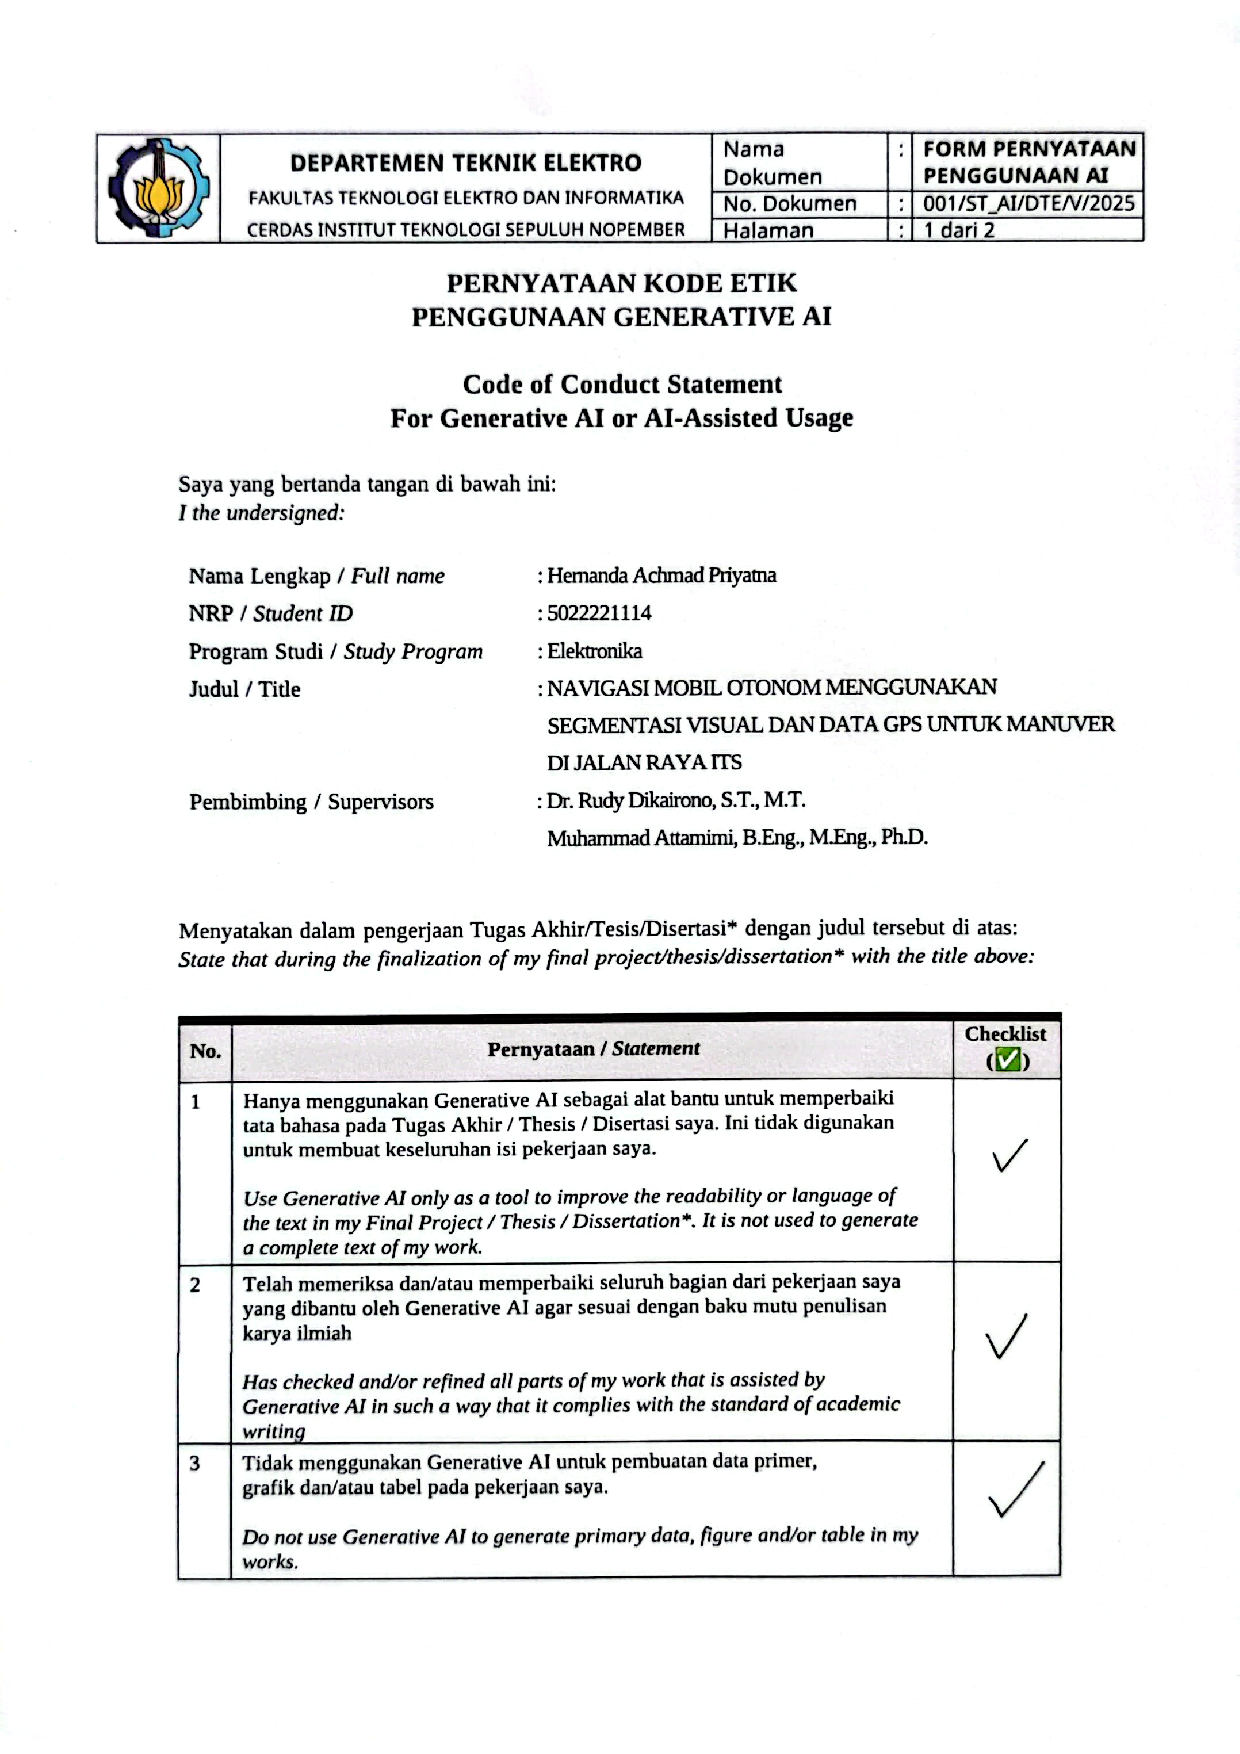
\includepdf[pages={1-2}]{lampiran/KodeEtikAI.pdf}
